\documentclass[a4paper,11pt]{article}
\usepackage[utf8]{inputenc}
\usepackage[french]{babel}
\usepackage{verbatim}
\usepackage{moreverb}
\usepackage{url}
\usepackage{graphicx}
\usepackage{fullpage}
\usepackage{float}


\begin{document}

\section{Interopérabilité et représentation des informations}


\subsection{Position du problème}


\paragraph*{}
Nous savons maintenant comment créer une architecture flexible grâce à REST, et nous connaissons un protocole applicatif adapté aux faibles ressources, et donc tout indiqué pour l'embarqué. Nous avons donc tout le nécessaire pour que nos applications puissent s'envoyer des messages, et pour créer facilement de nouvelles interfaces utilisant les services REST fournis.
Cependant, il y a encore un problème que nous n'avons pas abordé : nos applications doivent se comprendre. Si j'envoie une lettre en Français à un ami Chinois qui ne parle pas Français, la lettre arrivera sans problème mais ne lui sera d'aucune utilité. Il en va de même pour les applications : pour pouvoir échanger des données, l'application émettrice doit les représenter d'une manière compréhensible pour l'application réceptrice. Il est donc nécessaire de définir des normes, ou au minimum d'avoir des standards de fait, de préférence ouverts, concernant le format d'échange de données.\\
Aujourd'hui, deux formats sortent du lot pour remplir cette tâche : XML et JSON. Dans la suite, nous nous intéresseront à ces deux standards en essayant de montrer les forces et les faiblesses de chacun.



\subsection{XML : eXtensible Markup Language}

\subsubsection{Forme du langage}

La syntaxe d'XML contient deux éléments principaux permettant de structurer les informations : les balises, et les attributs. Cette syntaxe est en fait familière à toute personne ayant déjà manipulé du HTML \footnote{même si HTML n'est pas strictement un langage XML, excepté les deux versions de XHTML} : une balise peut contenir un ou plusieurs attributs dont chacun possède une valeur, puis on trouve le contenu, et enfin la balise fermante : 
\begin{verbatim}
	<balise attribut_1="valeur_1" attribut_2="valeur_2"> Contenu de la balise </balise>
\end{verbatim}

On peut organiser hiérarchiquement un document à l'aide de plusieurs balises différentes, en les imbriquant les unes dans les autres (en prenant soin de les fermer \emph{dans l'ordre}). On pourrait par exemple décrire un article de la manière suivante : 

\begin{verbatimtab}[4]
	<article auteur="Jean Dupont">
		<titre>Titre de l'article</titre>
		<sommaire>
			<chapitre id="1">Chapitre 1</chapitre>
			...
			<chapitre id="n">Chapitre n</chapitre>
		<sommaire>

		<contenu>
			<chapitre id="1">
				Contenu du chapitre, qui peut encore être divisé en sous sections,
				contenir des listes ...
			</chapitre>
			...
			<chapitre id="n">
				Contenu du chapitre
			</chapitre>
		</contenu>
	</aticle>
\end{verbatimtab}

\subsubsection{Pas un langage, un métalangage}
	\paragraph{}
	XML n'est en réalité pas un langage, mais un \emph{métalangage}. Il définit un certain nombre de règles, mais ne définit pas de vocabulaire (les mots-clés). Ainsi, dans l'exemple précédent, on utilise les mots \texttt{article}, \texttt{auteur}, \texttt{chapitre}, qui ne sont pas définis dans la norme XML. Tout langage XML est accompagné de la définition de son vocabulaire, définition qui peut prendre plusieurs formes, comme une \emph{DTD} \footnote{Document Type Definition} ou un \emph{schéma XML}.\\
	XML permet donc la définition d'un langage adapté à une utilisation spécifique, comme la représentation de pages web (XHTML\footnote{eXtensible HyperText Markup Language}), de documents bureautique (OpenDocument), ou encore d'images vectorielles (SVG\footnote{Scalable Vector Graphics}).
	Cette propriété rend XML très utile pour la conception de documents structurés de taille importante, et offre aux documents une forte valeur sémantique, utile par exemple pour des opérations d'indexation automatique. Par ailleurs, XML gère les \emph{espaces de noms}, permettant d'utiliser plusieurs vocabulaires différents dans un même document.


\subsubsection{Utilisation dans des applications REST}
\paragraph{Ce qui existe}
Un bon exemple d'implémentation de REST est le protocole HTTP, et l'une de ses utilisations grandissante est la méthode AJAX \footnote{Asynchronous JAvascript and XML}. Cette technologie, comme son nom l'indique, se repose à la base sur JavaScript et XML. Son principe est simple : un script JavaScript côté client envoie une requête HTTP à un serveur, qui lui renvoie les informations demandées en XML, puis le script utilise ces informations comme il le souhaite. Cette technique est souvent utilisée pour mettre à jour une page web sans avoir à la recharger entièrement, utile par exemple pour de l'auto-complétion dans un formulaire.


\paragraph{Limites}
Généralement, les retours venus du serveur sont assez réduits en volume (par exemple une liste ordonnée de 5 auto-complétions possibles). Il paraît alors un peu démesuré d'utiliser un format XML avec un vocabulaire précis (qui doit être connu du programme traitant les données), de la même manière qu'il serait démesuré de créer un document \LaTeX~pour faire sa liste de courses.\\
De plus, XML est relativement verbeux et peu économe en nombre de caractères nécessaires, notamment à cause des balises fermantes obligatoires, ce qui est gênant si l'on a des ressources limitées (n'oublions pas qu'un paquet CoAP doit obligatoirement tenir dans un paquet IP, une représentation des données trop peu compacte peut donc être handicapante).\\

Si XML est très adapté à la représentation de documents structurés, il semble l'être moins pour la représentation de petites quantités d'information, ce qui nous amène à considérer une représentation plus adaptée : JSON.



\subsection{JSON}

\paragraph*{}
JSON (prononcer \og Jason \fg), acronyme pour JAvascript Object Notation, propose une alternative agréable à XML pour la transmission de données. Apparu vers le début des années 2000, il a mis quelques années à se démocratiser, mais est aujourd'hui assez répandu et utilisé comme substitut à XML en AJAX

\subsection{Syntaxe de JSON}
JSON reprend la syntaxe du langage JavaScript, et se base sur deux structures de données : 
\begin{itemize}
	\item \textbf{L'Array} : un liste ordonnée de valeurs, entre crochets et séparées par des virgules :
		\begin{verbatimtab}[4]
		[Valeur_1, Valeur_2, ..., Valeur_n]
		\end{verbatimtab}
	\item \textbf{L'Object} : un tableau associatif ou hashtable, associant des clés (uniques) à des valeurs :
		\begin{verbatimtab}[4]

		{ "Clé_1" : Valeur_1,
		  "Clé_2" : Valeur_2,
		  ...
		  "Clé_n" : Valeur_n}
		\end{verbatimtab}
\end{itemize}

Une \emph{valeur} peut être un objet, un array, une chaine de caractères, un nombre flottant, ou encore les valeurs \texttt{true}, \texttt{false} et \texttt{null}.\\
Voici en détails la grammaire du langage JSON, présenté sous forme graphique, plus agréable à lire qu'une vraie grammaire EBNF (source : \url{json.org}) : 

\vspace{1\baselineskip}

\begin{figure}[H]
	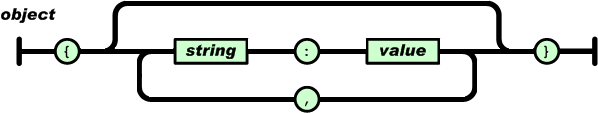
\includegraphics[width=15cm]{gramm_object} \\
	\caption{Grammaire des objets}
\end{figure}

\begin{figure}[H]
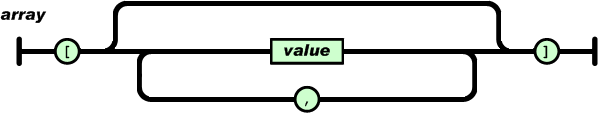
\includegraphics[width=15cm]{gramm_array}
	\caption{Grammaire des tableaux}
\end{figure}

\begin{figure}[H]
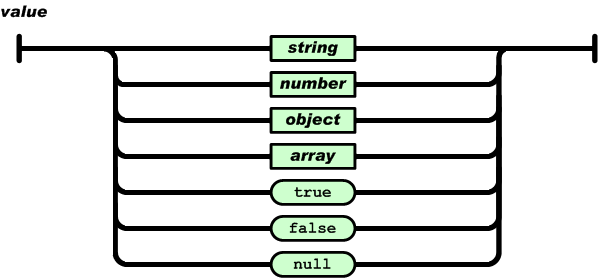
\includegraphics[width=15cm]{gramm_value}
	\caption{Grammaire des valeurs}
\end{figure}

\begin{figure}[H]
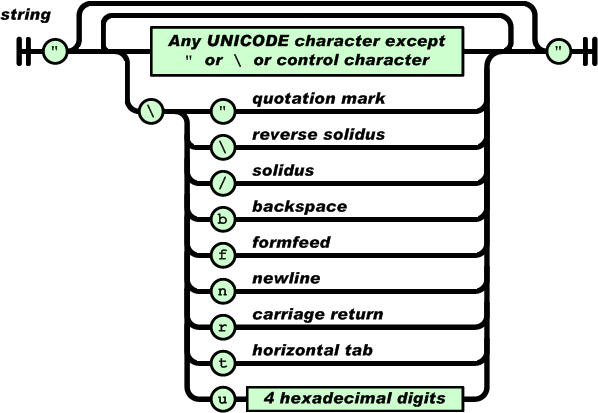
\includegraphics[width=15cm]{gramm_string}
	\caption{Grammaire des chaînes de caractères}
\end{figure}

\begin{figure}[H]
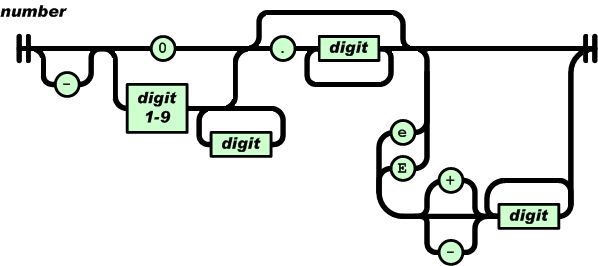
\includegraphics[width=15cm]{gramm_number}
	\caption{Grammaire des flottants}
\end{figure}


\subsection{Points forts}

\subsubsection{Parsage}
Nous venons de voir que la grammaire de JSON est très simple, puisque 5 règles suffisent à la décrire. Certaines seraient éclatées en plusieurs s'il fallait écrire une grammaire BNF lisible (la description des chaînes ou nombres ne se ferait peut-être pas en une seule règle), mais même dans ce cas, elles resteraient en nombre raisonnable. Même si ces cinq règles devaient se séparer en vingt lors de l'implémentation d'un analyseur syntaxique, on serait encore loin derrière les 89 utilisées pour décrire la grammaire d'XML \footnote{\url{http://www.w3.org/TR/REC-xml/}}.
Le parsage de données représentées en JSON apparaît donc comme étant plus léger, plus simple que pour du XML, ce qui est intéressant en particulier sur des systèmes à ressources limitées, comme les systèmes embarqués.

\subsubsection{Proximité avec les langages de programmation}
JSON se repose sur deux structures de données qui existent nativement dans un grand nombre de langages, ce qui permet de passer rapidement d'une donnée interne au programme à une donnée JSON à transmettre, et inversement. Le tableau est une structure native de presque tous les langages \og mainstream \fg~(tableaux de C, C++, Java, Python, \ldots).\\
En ce qui concerne les tableaux associatifs, ils sont natifs en Python (dictionnaires) ou Java (hashtable), et présents dans les conteneurs standards C++ (map). En ce qui concerne C, il n'y a rien de natif mais on trouve des implémentations de hashtables, notamment dans la glib. Cette proximité rend JSON adapté à la sérialisation d'objets, en particulier en JavaScript où la désérialisation consiste en une simple lecture de la chaîne de caractères\footnote{Cette pratique est cependant très peu sécurisée car du code malicieux pourrait facilement être exécuté, et ne devrait donc être utilisée que sur des systèmes dont on a le contrôle complet}, mais aussi pour de nombreux autres langages.


\subsection{JSON en pratique}
\paragraph{}
Pour ceux qui auraient d'ores et déjà décidé d'opter pour l'utilisation de JSON, voici quelques pistes pour démarrer plus vite.\\
\begin{description}
	\item[Parseurs JSON] : en bas de la page \url{json.org} se trouvent de nombreux liens vers des bibliothèques JSON en C, Python, C++, Lua, ou presque tout autre langage qui pourrait vous intéresser

	\item[Type MIME] : que ce soit pour HTTP ou CoAP, il est nécessaire de préciser dans l'en-tête du paquet que la charge utile est du JSON (pour que l'application distante puisse savoir comment la décoder). En HTTP, il s'agit de préciser le type MIME \texttt{application/json} à la section \texttt{Content-Type}.\\
		Pour CoAP, par souci d'économie de taille, les options ont un ordre fixe, et leurs valeurs sont encodées. On s'intéresse ici à l'option n\textdegree1 correspondant au champ Content-Type, dont la valeur correspondant au type application/json est \texttt{50}\footnote{Pour plus d'informations, se reporter au dernier draft de l'IETF : \url{http://tools.ietf.org/html/draft-ietf-core-coap-04}}.
		
	\item[Des hash-tables en C] : contrairement à Python et C++ (via la stdlib), le C ne possède pas de structure native pour les tableaux associatifs. Néanmoins, des implémentations existent, on peut notamment regarder du côté de la Glib \footnote{\url{http://library.gnome.org/devel/glib/stable/glib-Hash-Tables.html}}, ou simplement se débrouiller avec des \texttt{struct}.
\end{description}


\subsection{Références}
\begin{itemize}
	\item Le site officiel de JSON (avec une liste de bibliothèques en bas) :\url{http://library.gnome.org/devel/glib/stable/glib-Hash-Tables.html} \url{json.org}
	\item Le draft IETF de CoAP (expiration : janvier 2011), notamment pour le Content-Type : \url{http://tools.ietf.org/html/draft-ietf-core-coap-04}
	\item Des hashtables en C avec la Glib : \url{http://library.gnome.org/devel/glib/stable/glib-Hash-Tables.html}
	\item Une autre piste pour des hashtables en C : \url{http://www.mactech.com/articles/mactech/Vol.16/16.10/AssociativeArrays/index.html}
\end{itemize}
\end{document}
